\subsection{Closed-loop model of the system}
\label{sec:model}

Given that the Voronoi diagram is a conjunction of several line segments, without loss of generality, we assume that the waypoint lies on one such line segment.

We transform this waypoint along the coordinate axis where the Voronoi line segment is the x-axis, the rear wheel has coordinates $(x,y)$ and the orientation of the vehicle $\theta$ is w.r.t the line segment on the Voronoi diagram.
After the coordinate transformation, the orientation $\delta$ in this coordinate system will be
$$ tan(\delta) = \frac{2L}{\ell^2} (-\sqrt{\ell^2-y^2} \cdot sin(\theta)-y \cdot cos(\theta)). $$
Therefore,
\begin{align}
\dot{\theta} & = \frac{\displaystyle v}{\displaystyle L} \frac{\displaystyle 2L}{\displaystyle \ell^2} (-\sqrt{\ell^2-y^2} \cdot sin(\theta)-y \cdot cos(\theta)) \nonumber \\
& = \frac{\displaystyle 2v}{\displaystyle \ell^2} (-\sqrt{\ell^2-y^2} \cdot sin(\theta)-y \cdot cos(\theta))
\end{align}

The closed loop behavior of the vehicle dynamics is therefore given as:
\[
\begin{array}{l}
     \dot{x} = v \cdot cos(\theta) \\
     \dot{y} = v \cdot sin(\theta) \\
     \dot{\theta} = \frac{\displaystyle 2v}{\displaystyle \ell^2} (-\sqrt{\ell^2-y^2} \cdot sin(\theta)-y \cdot cos(\theta))
\end{array}
\]


% The above system is an open-loop system where $\delta$ is steering angle which is a control input. 
% %
% We close the loop by letting $\delta$ to be determined by the Pure Pursuit formula defined in (\ref{eqn:purepursuit}). 
% %
% In order to determine $\delta$, we need the coordinates of the goal point in the bicycle's frame. 
% %
% Since the plan is piecewise linear, $(g_x, g_y)$ defines a piecewise smooth curve in the bicycle's frame.
% %
% As a consequence, $\delta$ is a piecewise smooth function of time and is also be written as $\delta(t)$. 
% %
% The corners of this curve happen to be at times when the Pure Pursuit goal point moves from one line segment of the plan to the next. 
% %
% Therefore, we describe the dynamics of the system as a hybrid automaton where at each discrete mode, the goal point lies on a fixed linear piece of the plan. 
% %
% As a result, in each discrete mode, $\delta(t)$ will be a smooth function.

% Note that the formula for $\delta$ in (\ref{eqn:purepursuit}) was based on the coordinates of the goal point in the bicycle's local frame. 
% %
% However, the tracking path is described in the track's frame. 
% %
% Thus, the goal point is first described in the track's frame before we transform its coordinates to the bicycle's frame. 
% %
% For example, if the tracking path is the $x$-axis, the lookahead is $\ell$, and the car is within $\ell$ distance of the $x$-axis, then
% $$ tan(\delta) = \frac{2L}{\ell^2} (-\sqrt{\ell^2-y^2} \cdot sin(\theta)-y \cdot cos(\theta)). $$
% Therefore,
% \begin{align}
% \dot{\theta} & = \frac{\displaystyle v}{\displaystyle L} \frac{\displaystyle 2L}{\displaystyle \ell^2} (-\sqrt{\ell^2-y^2} \cdot sin(\theta)-y \cdot cos(\theta)) \nonumber \\
% & = \frac{\displaystyle 2v}{\displaystyle \ell^2} (-\sqrt{\ell^2-y^2} \cdot sin(\theta)-y \cdot cos(\theta))
% \end{align}
% % $$ \begin{array}{rcl}
% %   \dot{\theta} & = & \frac{\displaystyle v}{\displaystyle L} \frac{\displaystyle 2L}{\displaystyle \ell^2} (-\sqrt{\ell^2-y^2} \cdot sin(\theta)-y \cdot cos(\theta))  \\
% %      & = & \frac{\displaystyle 2v}{\displaystyle \ell^2} (-\sqrt{\ell^2-y^2} \cdot sin(\theta)-y \cdot cos(\theta))
% % \end{array}
% % $$
% which closes the control loop (assuming $v$ is a function of the state). 
% %
% Adding $v$ to the model explicitly models the dynamic interaction between the set point and the state of the vehicle.

Notice that this closed loop behavior is accurate as long as the way-point lies on the same line segment.
%
When the vehicle makes progress, the lookahead circle would intersect with a different line segment on the Voronoi diagram.
%
As a result, the way-point as well as coordinate system for modeling the evolution of vehicle state change.
%
We model this behavior as a hybrid automaton for a given circuit.

\begin{figure}
\centering
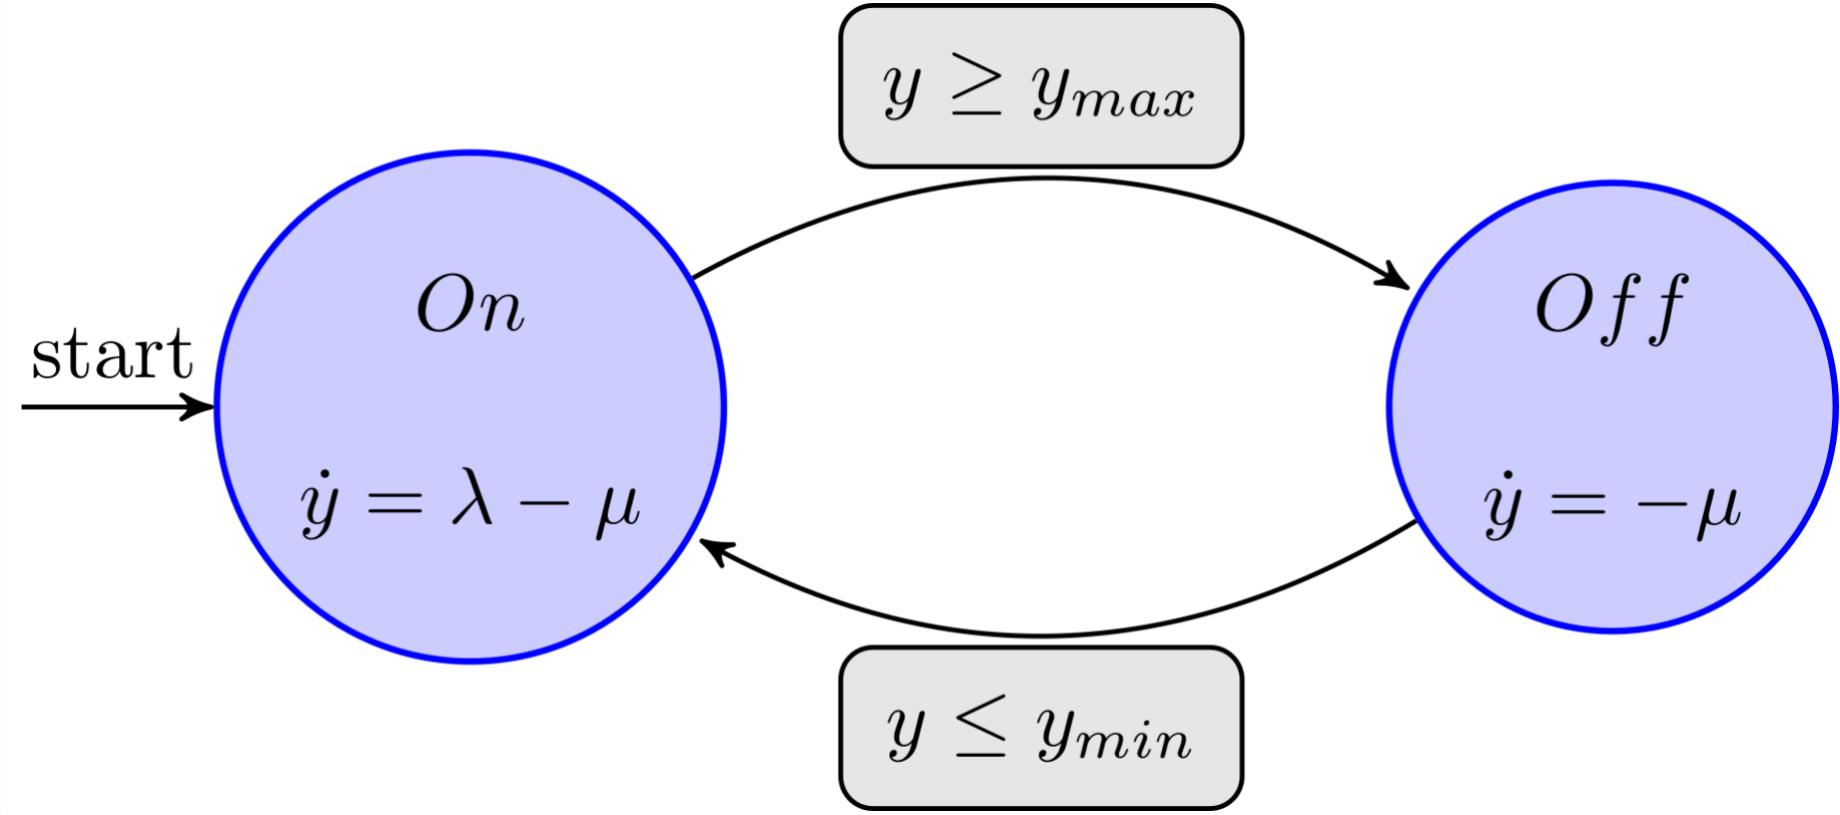
\includegraphics[width=0.8\linewidth]{Figures/hybrid-automaton.jpeg}
\caption{Hybrid automaton of a multiple-tank system.}
\label{fig:ha}
\end{figure}

% \begin{definition} 
% A hybrid automata is defined as a tuple $\langle Mod, X, E, Flows \rangle$ where
% \begin{itemize}
%     \item \textbf{$Modes$} is the set of discrete modes,
%     \item \textbf{$X$} is the state space,
%     \item \textbf{$E$} is the set of discrete transitions among modes, and
%     \item \textbf{$Flows$} describes the evolution of the system in each mode.
% \end{itemize}
% \end{definition}

\begin{definition}
\label{def:hybridSystem}
 A \emph{hybrid automaton} is a mathematical model of a hybrid system $H$ which is defined as a tuple $\langle Loc, X, Flow, Inv, E, G, Rst \rangle$ where:
%  \vspace{-0.2cm}
\begin{description}
\item[$Loc$] is a finite set of locations.
\item[$X$] $\subseteq \mathbb{R}^n$ is the state space of the behaviors.
\item[$Flow$] $: Loc \rightarrow \mathcal{F}(X)$ assigns a  differential equation $\mathcal{F}$ over $X$ to each location of the hybrid automaton.
\item[$Inv$] $: Loc \rightarrow 2^{\mathbb{R}^n}$ assigns an invariant set of states to each location.
\item[$E$] $\subseteq Loc \times Loc$ is the set of discrete transitions.
\item[$G$] $: E \rightarrow 2^{\mathbb{R}^n}$ defines the set of states for a enabled discrete transition.
\item[$Rst$] $: E \times 2^{\mathbb{R}^n} \rightarrow 2^{\mathbb{R}^n}$ determines the set of states after a discrete  transition is taken.
\end{description}
% \vspace{-0.2cm}
A hybrid system is \emph{linear} if each $\mathcal{F}$ is a linear differential equation and its invariants and guards are given as the conjunction of linear constraints.
\end{definition}

% Often, $Flows$ are described as a collection of nonlinear differential equations, one for each mode.
%
Each discrete transition $e \doteq (loc, loc') \in E$ among locations  $loc, loc' \in Loc$ of the hybrid automata has an associated $G(e)$ condition. The hybrid automaton can take the transition $e$ only when the state of the trajectory satisfies $G(e)$.
%
Additionally, after taking the transition $e$, the state of the system changes from its current state $x \in \mathbb{R}^n$ to a new state $x'$ defined according to a reset function $x' = Rst(e,x)$.
%

% In the case of the vehicle following the waypoint on Voronoi diagram, when a new line segment is encountered by the lookahead circle, the change of basis variables (alignment of the x-axis along the new segment) is the reset function.
%
As the vehicle following a way-point on Voronoi diagram encounters a new line segment, a discrete transition is enabled. Notice that the set of states that take this transition as defined by it's guard lies on a circle of radius $\ell$ from an end point of the new line segment.
%
This set is a non-convex set.
%
Performing reachability analysis with non-convex guard conditions is very challenging.
%
We, therefore, compute a convex overapproximation of the original guard as shown in Fig.~\ref{fig:guard_inv_approx}. This abstraction of the hybrid automaton admits more behaviors than the original model, but is easier to analyze.
%
% More specifically, we allow the hybrid automata to non-deterministically take a transition whenever the vehicle enters the convex overapproximation of the original guard condition.
%
Since this guard over-approximation strictly increases the set of possible states that take the discrete transition, it is easy to observe that the abstract hybrid automaton includes all the behaviors of the original model.
%
% Illustration of the abstraction of the guard condition for hybrid automata modeling the behavior of the vehicle is given in Figure~\ref{fig:guard_inv_approx}.
%
%
% Given a circuit, we construct the hybrid automata model of the vehicle moving in the lap using our Voronoi planning and pure pursuit control algorithm.
%
We next discuss the techniques for proving the safety and progress properties of the vehicle.

% When the vehicle encounters a new line segment in the roadmap, the behavior of the model changes as the set point now evolves on the new line segment.
% %
% This switching behavior is modelled as a hybrid automata.
% %
% The exact guard condition for switching is non-convex and hence reachable set computation tools cannot analyze such models.

% To make our analysis simpler, we overapproximate the guard set to allow for additional behaviors.
% The simplified guard and invariant of a location which corresponds to a pair of way points are represented in Fig.~\ref{fig:guard_inv_approx}.


% One of the challenging parts of defining the hybrid automaton is that
% the tracking path as defined by the Voronoi diagram consists of not only line segments
% but also parabolic curve segments (Figure ~\ref{fig:rect_voronoi}).
% Furthermore,
% at any moment in time,
% only some of the walls are visible to the car. Consequently, the Voronoi diagram changes as the car sees more walls (Figure \ref{fig:vd_turn}).


% \begin{figure}
% \centering
% \subfigure[]{%
% 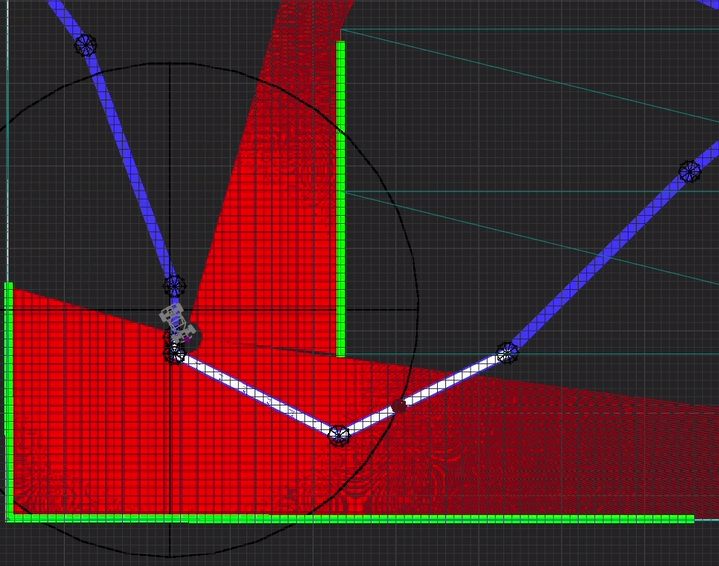
\includegraphics[width=42mm]{Figures/before_turn.png}%
% \label{fig:vd_beforeTurn}%
% }\quad
% \subfigure[]{%
% 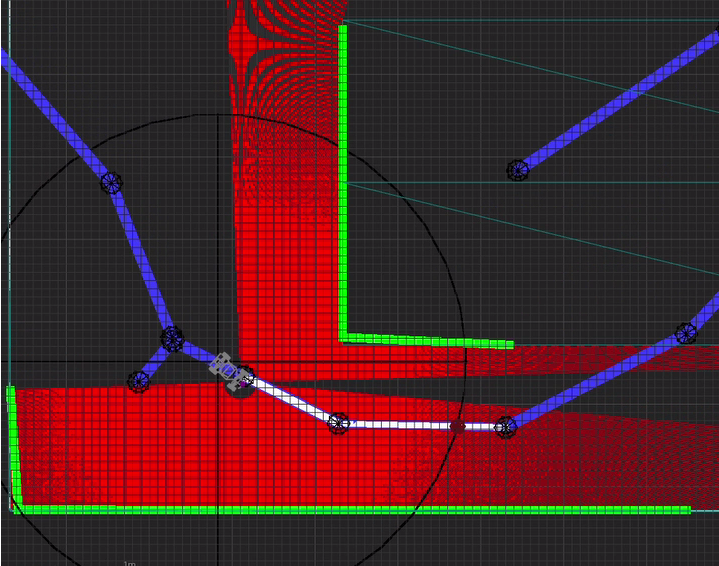
\includegraphics[width=42mm]{Figures/inside_turn.png}%
% \label{fig:vd_afterTurn}%
% }
% \caption{Roadmap around a corner: A big lookahead can create dicontinuous goal for Pure Pursuit.
% (a) Before the turn.
% (b) Inside the turn.}
% \label{fig:vd_turn}
% \end{figure}

% This requires that we manually analyze the track to see what discrete modes are needed.
% Additionally, if Pure Pursuit controller is commanding a steering angle beyond the maximum permissible steering angle of the car, the system should go to a new discrete mode where the steering angle is fixed at that maximum. In future, we intend to automate the construction of the hybrid automaton based on the geometry of the track and steering limitations of the car.

% In this paper we study tracks with moderate curvature and small uncertainty in the initial set so that steering will not be saturated in the verification. Also we keep the lookahead distance of the Pure Pursuit controller small enough to avoid the problem encountered in Fig~\ref{fig:vd_turn}.

\begin{figure}
\centering
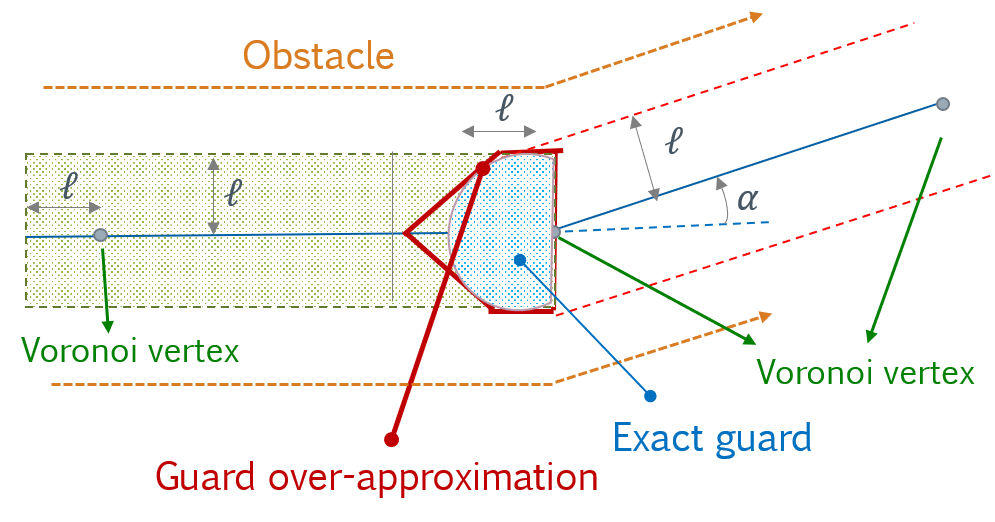
\includegraphics[width=0.8\linewidth]{Figures/rss2021-guard-approximate.png}
\caption{Over-approximation of guard.  $l$ is the look ahead distance of the car. The original exact guard is circular and we linearize it as a convex polytope that is defined using linear constraints.}
\label{fig:guard_inv_approx}
\end{figure}


% \begin{itemize}
% \item Removed the formal definition of hybrid automata.
% \item Add a reduced version of hybrid automata.
% \item Show when do the transitions happen.
% \end{itemize}